\chapter{Appendix}

% TODO: show parameters for sklearn models

\section{Sklearn Model Parameters for Single Station Interpolation}
\label{appendix: sklearn ml parameters single station}

\begin{lstlisting}[language=Python, caption=Random Forest Regressor Parameters]
class sklearn.ensemble.RandomForestRegressor(n_estimators=200,
*, criterion='squared_error', max_depth=None, min_samples_split=2,
min_samples_leaf=1, min_weight_fraction_leaf=0.0, max_features=1.0,
max_leaf_nodes=None, min_impurity_decrease=0.0, bootstrap=True,
oob_score=False, n_jobs=None, random_state=None, verbose=0,
warm_start=False, ccp_alpha=0.0, max_samples=None)
\end{lstlisting}

The number of trees was increaed from 100 to 200 to increase the performance.

\begin{lstlisting}[language=Python, caption=Histogram-based Gradient Boosting Parameters]
class sklearn.ensemble.HistGradientBoostingRegressor
(loss='squared_error', *, quantile=None, learning_rate=0.1,
max_iter=200, max_leaf_nodes=31, max_depth=None, min_samples_leaf=20,
l2_regularization=0.0, max_bins=255, categorical_features=None,
monotonic_cst=None, interaction_cst=None, warm_start=False,
early_stopping='auto', scoring='loss', validation_fraction=0.1,
n_iter_no_change=10, tol=1e-07, verbose=0, random_state=42)
\end{lstlisting}

The number of max iterations was increased from the default value of 100 to 200 to improve the performance of the model and the random state was set to 42 so all interations yield the same result.

\section{Feature Engineering}

\begin{lstlisting}[language=Python, caption=Timestamp to Sinus Curve Feature, label=lst: timestamp to sin]
    # Convert datetime64 timestamp hours and minutes to circle angle
    filtered_gdf['time'] = filtered_gdf['time'].apply(lambda x: (x.hour * 60 + x.minute) * 2 * np.pi / (24 * 60))
    filtered_gdf.rename(columns={'time': 'time_angle'}, inplace=True)

    # Calculate continuous representation of time as an angle in radians
    filtered_gdf['sin_time'] = np.sin(filtered_gdf['time_angle'])
\end{lstlisting}

\section{Histogram-based Gradient Boosting Single Location Interpolation}

\subsubsection{List of stations for minimum distance between stations}
\label{appendix stations for minimum distance between stations}

The list of stations for the minimum distance between stations is the following by their Netatmo station id:

\begin{itemize}
    \item 70:ee:50:83:b1:e2 
    \item 70:ee:50:16:16:ce
    \item 70:ee:50:5e:d4:16
    \item 70:ee:50:00:d3:96
    \item 70:ee:50:6b:5f:50
    \item 70:ee:50:00:d1:1c
    \item 70:ee:50:5f:51:a0
    \item 70:ee:50:6b:97:86
    \item 70:ee:50:28:f2:ca
    \item 70:ee:50:58:e8:70
\end{itemize}

The locations of the stations are presented in Figure~\ref{fig:eval_hamburg_locations_point_histb_10_map}.

\begin{figure}[ht]
    \centering
    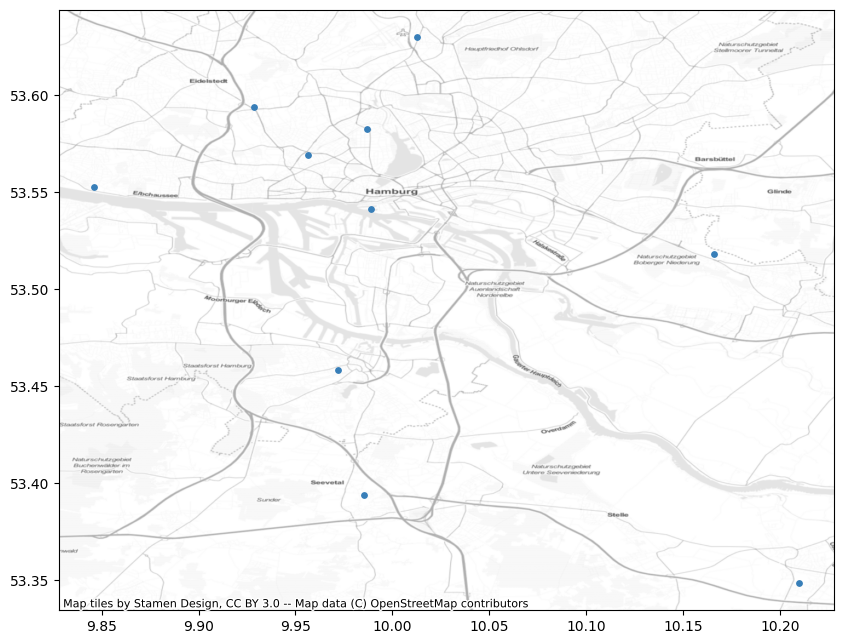
\includegraphics[width=1\textwidth]{images/eval_hamburg_locations_point_histb_10_map.png}
    \caption{Netatmo Stations for Minimum Distance Between Stations, Hamburg}
    \label{fig:eval_hamburg_locations_point_histb_10_map}
\end{figure}